\subsection*{Partie A}

\begin{enumerate}
	\item $-x^2 + 7x + 8 =0$ admet $-1$ comme solution évidente. L'autre solution de l'équation du second degré est donc $8$.

Le trinôme est négatif (du signe du coefficient de $x^2$), sauf entre les racines, d'où le tableau de signes  de $x\longmapsto -x^2 + 7x + 8 $ :
	
	\begin{tikzpicture}
	\tkzTabInit[lgt=5.5,espcl=2]
	{$x$
	/1,
	signe de $-x^2+7x+8$
	/1
	}
	{$-\infty$ , $-1$ , $8$ , $+\infty$}
	\tkzTabLine{, - , z , + , z, -, }
	\end{tikzpicture}
	
L'ensemble des solutions de l'inéquation 	$-x^2 + 7x + 8 \geqslant 0$ sur $\R$ est l'intervalle $\left[-1~;~8\right]$
	
	\item Pour tout nombre réel $x$ appartenant à l'intervalle $\left]0~;~8\right]$, $-x^2 + 7x + 8 \geqslant 0$. D'où en ajoutant 1 à chaque membre $-x^2 + 7x + 9 \geqslant 1$.

	Comme la fonction logarithme népérien est une fonction croissante on a pour tout  $x$ appartenant à $\left]0~;~8\right]$, $\ln\left(- x^2 + 7x + 9\right) \geqslant \ln(1)$. C'est à dire $\ln\left(- x^2 + 7x + 9\right) \geqslant 0$.

Pour tout $x$ appartenant à $\left]0~;~8\right]$, $x>0$ et  $10\ln\left(-x^2 + 7x + 9\right) \geqslant 0$, donc $f(x) = \dfrac{10\ln\left(-x^2 + 7x + 9\right)}{x} \geqslant 0$.

	\item Sur l'intervalle $[0~;~8]$ la courbe représentative est au dessus de l'axe des abscisses.
	
\end{enumerate}

\subsection*{Partie B}

\begin{enumerate}
	\item Pour $x\in \left]0~;~8\right]$, M$\left(x,\dfrac{10\ln\left(-x^2 + 7x + 9\right)}{x}\right)$ et donc N$\left(x,0\right)$ et P$\left(0,\dfrac{10\ln\left(-x^2 + 7x + 9\right)}{x}\right)$.
	\item Comme pour $x\in \left]0~;~8\right]$, l'abscisse de N est positive et l'ordonnée de P est positive. On peut écrire ON$=x$ et OP$=\dfrac{10\ln\left(-x^2 + 7x + 9\right)}{x}$.
	
	L'aire de ONMP vaut $\text{ON}\times\text{OP}$ donc : 
	
	$\forall x \in \left]0~;~8\right]\quad \mathcal{A}(x) = x\times \dfrac{10\ln\left(-x^2 + 7x + 9\right)}{x} = 10\ln\left(-x^2 + 7x + 9\right)$
	\item Sur $\left]0~;~8\right[$, $-x^2 + 7x + 9 > 0$ donc $\mathcal{A}$ est une fonction dérivable de la variable $x$ sur $\left]0~;~8\right[$ comme composée de fonction définies et dérivables. 
	
	$\forall x\in \left]0~;~8\right[$, $\mathcal{A}'(x) = 10\times \dfrac{-2x + 7}{-x^2 + 7x +9}$.
	
	S'il existe $x\in \left]0~;~8\right[$ telle que $\mathcal{A}(x)$ soit maximale, il faut que $\mathcal{A}'(x) = 0$
	
	Pour $x\in \left]0~;~8\right[$, $-x^2 + 7x +9 > 0 $,  $\mathcal{A}'(x)$ est donc du signe de $-2x + 7$.
	
	$
	\begin{array}{ccc}
	\mathcal{A}'(x) \geqslant 0 &\iff& -2x + 7 \geqslant 0 \\
	\mathcal{A}'(x) \geqslant 0 &\iff& x \leqslant \dfrac{7}{2} \\
	\end{array}
	$

	$\mathcal{A}$ est croissante sur $\left]0~;~\dfrac{7}{2}\right[$ et décroissante sur  $\left]\dfrac{7}{2}~;~8\right[$.
	
	La dérivée s'annule en $\dfrac{7}{2}$, en étant positive avant puis négative après, donc la fonction $\mathcal{A}$ a un maximum sur $]0~;~8[$, : 
	
	$\mathcal{A}\left(\dfrac{7}{2}\right) = 10\ln(17)+ 10\ln(5)-20\ln(2) \approx \np{30.56}$
	
	\end{enumerate}
	
\subsection*{Partie C}

\begin{enumerate}
	\item \ {} 
	
\begin{center}
\begin{lstlisting}[language=python,frame=single, escapechar=|, numbers=left]
from math import *	

def A(x):
	return 10*log(-1 * x**2 + 7*x + 9)
	
def pluspetitevaleur(k):
	x = 3.5
	while A(x) > k:
		x = x + 0.1
	return x	

\end{lstlisting}
\end{center}
	
	\item
	\begin{lstlisting}[language=python]
>>>pluspetitevaleur(30)
4.599999999999998
\end{lstlisting}
	
	\item Lorsque $k=35$, la condition \verb!A(x) > 35! n'est pas vérifiée donc le contenu de la boucle n'est pas exécuté. L'appel \verb!pluspetitevaleur(35)! renvoie \verb!3.5!.
\end{enumerate}
